% Options for packages loaded elsewhere
\PassOptionsToPackage{unicode}{hyperref}
\PassOptionsToPackage{hyphens}{url}
\PassOptionsToPackage{dvipsnames,svgnames,x11names}{xcolor}
%
\documentclass[
  number]{elsarticle}

\usepackage{amsmath,amssymb}
\usepackage{iftex}
\ifPDFTeX
  \usepackage[T1]{fontenc}
  \usepackage[utf8]{inputenc}
  \usepackage{textcomp} % provide euro and other symbols
\else % if luatex or xetex
  \usepackage{unicode-math}
  \defaultfontfeatures{Scale=MatchLowercase}
  \defaultfontfeatures[\rmfamily]{Ligatures=TeX,Scale=1}
\fi
\usepackage{lmodern}
\ifPDFTeX\else  
    % xetex/luatex font selection
\fi
% Use upquote if available, for straight quotes in verbatim environments
\IfFileExists{upquote.sty}{\usepackage{upquote}}{}
\IfFileExists{microtype.sty}{% use microtype if available
  \usepackage[]{microtype}
  \UseMicrotypeSet[protrusion]{basicmath} % disable protrusion for tt fonts
}{}
\makeatletter
\@ifundefined{KOMAClassName}{% if non-KOMA class
  \IfFileExists{parskip.sty}{%
    \usepackage{parskip}
  }{% else
    \setlength{\parindent}{0pt}
    \setlength{\parskip}{6pt plus 2pt minus 1pt}}
}{% if KOMA class
  \KOMAoptions{parskip=half}}
\makeatother
\usepackage{xcolor}
\setlength{\emergencystretch}{3em} % prevent overfull lines
\setcounter{secnumdepth}{5}
% Make \paragraph and \subparagraph free-standing
\makeatletter
\ifx\paragraph\undefined\else
  \let\oldparagraph\paragraph
  \renewcommand{\paragraph}{
    \@ifstar
      \xxxParagraphStar
      \xxxParagraphNoStar
  }
  \newcommand{\xxxParagraphStar}[1]{\oldparagraph*{#1}\mbox{}}
  \newcommand{\xxxParagraphNoStar}[1]{\oldparagraph{#1}\mbox{}}
\fi
\ifx\subparagraph\undefined\else
  \let\oldsubparagraph\subparagraph
  \renewcommand{\subparagraph}{
    \@ifstar
      \xxxSubParagraphStar
      \xxxSubParagraphNoStar
  }
  \newcommand{\xxxSubParagraphStar}[1]{\oldsubparagraph*{#1}\mbox{}}
  \newcommand{\xxxSubParagraphNoStar}[1]{\oldsubparagraph{#1}\mbox{}}
\fi
\makeatother

\usepackage{color}
\usepackage{fancyvrb}
\newcommand{\VerbBar}{|}
\newcommand{\VERB}{\Verb[commandchars=\\\{\}]}
\DefineVerbatimEnvironment{Highlighting}{Verbatim}{commandchars=\\\{\}}
% Add ',fontsize=\small' for more characters per line
\usepackage{framed}
\definecolor{shadecolor}{RGB}{241,243,245}
\newenvironment{Shaded}{\begin{snugshade}}{\end{snugshade}}
\newcommand{\AlertTok}[1]{\textcolor[rgb]{0.68,0.00,0.00}{#1}}
\newcommand{\AnnotationTok}[1]{\textcolor[rgb]{0.37,0.37,0.37}{#1}}
\newcommand{\AttributeTok}[1]{\textcolor[rgb]{0.40,0.45,0.13}{#1}}
\newcommand{\BaseNTok}[1]{\textcolor[rgb]{0.68,0.00,0.00}{#1}}
\newcommand{\BuiltInTok}[1]{\textcolor[rgb]{0.00,0.23,0.31}{#1}}
\newcommand{\CharTok}[1]{\textcolor[rgb]{0.13,0.47,0.30}{#1}}
\newcommand{\CommentTok}[1]{\textcolor[rgb]{0.37,0.37,0.37}{#1}}
\newcommand{\CommentVarTok}[1]{\textcolor[rgb]{0.37,0.37,0.37}{\textit{#1}}}
\newcommand{\ConstantTok}[1]{\textcolor[rgb]{0.56,0.35,0.01}{#1}}
\newcommand{\ControlFlowTok}[1]{\textcolor[rgb]{0.00,0.23,0.31}{\textbf{#1}}}
\newcommand{\DataTypeTok}[1]{\textcolor[rgb]{0.68,0.00,0.00}{#1}}
\newcommand{\DecValTok}[1]{\textcolor[rgb]{0.68,0.00,0.00}{#1}}
\newcommand{\DocumentationTok}[1]{\textcolor[rgb]{0.37,0.37,0.37}{\textit{#1}}}
\newcommand{\ErrorTok}[1]{\textcolor[rgb]{0.68,0.00,0.00}{#1}}
\newcommand{\ExtensionTok}[1]{\textcolor[rgb]{0.00,0.23,0.31}{#1}}
\newcommand{\FloatTok}[1]{\textcolor[rgb]{0.68,0.00,0.00}{#1}}
\newcommand{\FunctionTok}[1]{\textcolor[rgb]{0.28,0.35,0.67}{#1}}
\newcommand{\ImportTok}[1]{\textcolor[rgb]{0.00,0.46,0.62}{#1}}
\newcommand{\InformationTok}[1]{\textcolor[rgb]{0.37,0.37,0.37}{#1}}
\newcommand{\KeywordTok}[1]{\textcolor[rgb]{0.00,0.23,0.31}{\textbf{#1}}}
\newcommand{\NormalTok}[1]{\textcolor[rgb]{0.00,0.23,0.31}{#1}}
\newcommand{\OperatorTok}[1]{\textcolor[rgb]{0.37,0.37,0.37}{#1}}
\newcommand{\OtherTok}[1]{\textcolor[rgb]{0.00,0.23,0.31}{#1}}
\newcommand{\PreprocessorTok}[1]{\textcolor[rgb]{0.68,0.00,0.00}{#1}}
\newcommand{\RegionMarkerTok}[1]{\textcolor[rgb]{0.00,0.23,0.31}{#1}}
\newcommand{\SpecialCharTok}[1]{\textcolor[rgb]{0.37,0.37,0.37}{#1}}
\newcommand{\SpecialStringTok}[1]{\textcolor[rgb]{0.13,0.47,0.30}{#1}}
\newcommand{\StringTok}[1]{\textcolor[rgb]{0.13,0.47,0.30}{#1}}
\newcommand{\VariableTok}[1]{\textcolor[rgb]{0.07,0.07,0.07}{#1}}
\newcommand{\VerbatimStringTok}[1]{\textcolor[rgb]{0.13,0.47,0.30}{#1}}
\newcommand{\WarningTok}[1]{\textcolor[rgb]{0.37,0.37,0.37}{\textit{#1}}}

\providecommand{\tightlist}{%
  \setlength{\itemsep}{0pt}\setlength{\parskip}{0pt}}\usepackage{longtable,booktabs,array}
\usepackage{calc} % for calculating minipage widths
% Correct order of tables after \paragraph or \subparagraph
\usepackage{etoolbox}
\makeatletter
\patchcmd\longtable{\par}{\if@noskipsec\mbox{}\fi\par}{}{}
\makeatother
% Allow footnotes in longtable head/foot
\IfFileExists{footnotehyper.sty}{\usepackage{footnotehyper}}{\usepackage{footnote}}
\makesavenoteenv{longtable}
\usepackage{graphicx}
\makeatletter
\newsavebox\pandoc@box
\newcommand*\pandocbounded[1]{% scales image to fit in text height/width
  \sbox\pandoc@box{#1}%
  \Gscale@div\@tempa{\textheight}{\dimexpr\ht\pandoc@box+\dp\pandoc@box\relax}%
  \Gscale@div\@tempb{\linewidth}{\wd\pandoc@box}%
  \ifdim\@tempb\p@<\@tempa\p@\let\@tempa\@tempb\fi% select the smaller of both
  \ifdim\@tempa\p@<\p@\scalebox{\@tempa}{\usebox\pandoc@box}%
  \else\usebox{\pandoc@box}%
  \fi%
}
% Set default figure placement to htbp
\def\fps@figure{htbp}
\makeatother

\makeatletter
\@ifpackageloaded{caption}{}{\usepackage{caption}}
\AtBeginDocument{%
\ifdefined\contentsname
  \renewcommand*\contentsname{Table of contents}
\else
  \newcommand\contentsname{Table of contents}
\fi
\ifdefined\listfigurename
  \renewcommand*\listfigurename{List of Figures}
\else
  \newcommand\listfigurename{List of Figures}
\fi
\ifdefined\listtablename
  \renewcommand*\listtablename{List of Tables}
\else
  \newcommand\listtablename{List of Tables}
\fi
\ifdefined\figurename
  \renewcommand*\figurename{Figure}
\else
  \newcommand\figurename{Figure}
\fi
\ifdefined\tablename
  \renewcommand*\tablename{Table}
\else
  \newcommand\tablename{Table}
\fi
}
\@ifpackageloaded{float}{}{\usepackage{float}}
\floatstyle{ruled}
\@ifundefined{c@chapter}{\newfloat{codelisting}{h}{lop}}{\newfloat{codelisting}{h}{lop}[chapter]}
\floatname{codelisting}{Listing}
\newcommand*\listoflistings{\listof{codelisting}{List of Listings}}
\makeatother
\makeatletter
\makeatother
\makeatletter
\@ifpackageloaded{caption}{}{\usepackage{caption}}
\@ifpackageloaded{subcaption}{}{\usepackage{subcaption}}
\makeatother

\usepackage[]{natbib}
\bibliographystyle{plainnat}
\usepackage{bookmark}

\IfFileExists{xurl.sty}{\usepackage{xurl}}{} % add URL line breaks if available
\urlstyle{same} % disable monospaced font for URLs
\hypersetup{
  pdftitle={pre-covid model},
  colorlinks=true,
  linkcolor={blue},
  filecolor={Maroon},
  citecolor={Blue},
  urlcolor={Blue},
  pdfcreator={LaTeX via pandoc}}


\setlength{\parindent}{6pt}
\begin{document}

\begin{frontmatter}
\title{pre-covid model}


\cortext[cor1]{Corresponding author}
        





\end{frontmatter}
    

We will build a model for emergencies appointements for both Vila do
Conde and Barcelos. We will then use this model to replace the covid
period for our future analysis.

\begin{Shaded}
\begin{Highlighting}[]
\NormalTok{df }\OtherTok{\textless{}{-}} \FunctionTok{read\_csv}\NormalTok{(}\StringTok{"../data/transformed/tratadas\_emergencias.csv"}\NormalTok{)}
\end{Highlighting}
\end{Shaded}

\begin{verbatim}
Rows: 282 Columns: 6
-- Column specification --------------------------------------------------------
Delimiter: ","
chr  (2): instituicao, unidade_saude
dbl  (3): urgencias_geral, year, urgencias_mensais
date (1): data

i Use `spec()` to retrieve the full column specification for this data.
i Specify the column types or set `show_col_types = FALSE` to quiet this message.
\end{verbatim}

\begin{Shaded}
\begin{Highlighting}[]
\NormalTok{df }\OtherTok{\textless{}{-}}\NormalTok{ df }\SpecialCharTok{\%\textgreater{}\%} \FunctionTok{filter}\NormalTok{(data }\SpecialCharTok{\textless{}} \StringTok{"2020{-}01{-}01"}\NormalTok{) }

\NormalTok{df }\OtherTok{\textless{}{-}}\NormalTok{ df }\SpecialCharTok{\%\textgreater{}\%} 
    \FunctionTok{group\_by}\NormalTok{(unidade\_saude) }\SpecialCharTok{\%\textgreater{}\%} 
    \FunctionTok{nest}\NormalTok{()}
\end{Highlighting}
\end{Shaded}

\subsection{Vila do Conde}\label{vila-do-conde}

\begin{Shaded}
\begin{Highlighting}[]
\NormalTok{df }\SpecialCharTok{\%\textgreater{}\%} 
    \FunctionTok{filter}\NormalTok{(unidade\_saude }\SpecialCharTok{==} \StringTok{"Vila do Conde"}\NormalTok{) }\SpecialCharTok{\%\textgreater{}\%}
    \FunctionTok{unnest}\NormalTok{(}\AttributeTok{cols =} \FunctionTok{c}\NormalTok{(data)) }\SpecialCharTok{\%\textgreater{}\%}  
    \FunctionTok{ggplot}\NormalTok{(}\FunctionTok{aes}\NormalTok{(}\AttributeTok{x =}\NormalTok{ data, }\AttributeTok{y =}\NormalTok{ urgencias\_mensais )) }\SpecialCharTok{+}
    \FunctionTok{geom\_line}\NormalTok{(}\AttributeTok{color =} \StringTok{"blue"}\NormalTok{) }\SpecialCharTok{+}
    \FunctionTok{theme\_classic}\NormalTok{() }\SpecialCharTok{+}
    \FunctionTok{scale\_x\_date}\NormalTok{(}\AttributeTok{date\_breaks =} \StringTok{"1 year"}\NormalTok{, }\AttributeTok{date\_labels =} \StringTok{"\%m \%Y"}\NormalTok{) }\SpecialCharTok{+}
    \FunctionTok{theme}\NormalTok{(}\AttributeTok{axis.text.x =} \FunctionTok{element\_text}\NormalTok{(}\AttributeTok{angle =} \DecValTok{90}\NormalTok{, }\AttributeTok{hjust =} \DecValTok{1}\NormalTok{))}
\end{Highlighting}
\end{Shaded}

\pandocbounded{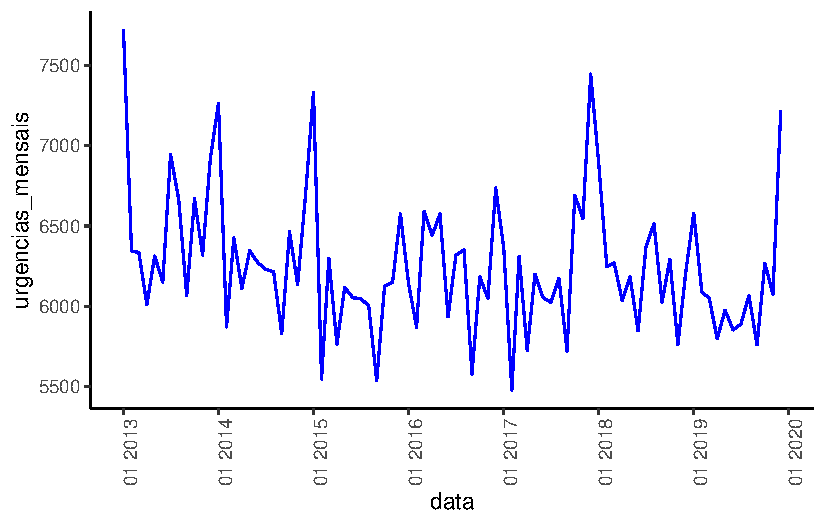
\includegraphics[keepaspectratio]{pre-covid-model_files/figure-pdf/unnamed-chunk-2-1.pdf}}

\begin{Shaded}
\begin{Highlighting}[]
\NormalTok{df }\SpecialCharTok{\%\textgreater{}\%} 
    \FunctionTok{filter}\NormalTok{(unidade\_saude }\SpecialCharTok{==} \StringTok{"Vila do Conde"}\NormalTok{) }\SpecialCharTok{\%\textgreater{}\%}
    \FunctionTok{unnest}\NormalTok{(}\AttributeTok{cols =} \FunctionTok{c}\NormalTok{(data)) }\SpecialCharTok{\%\textgreater{}\%} 
    \FunctionTok{pull}\NormalTok{(urgencias\_mensais) }\SpecialCharTok{\%\textgreater{}\%} 
    \FunctionTok{acf}\NormalTok{(}\AttributeTok{lag.max =} \DecValTok{50}\NormalTok{)}
\end{Highlighting}
\end{Shaded}

\pandocbounded{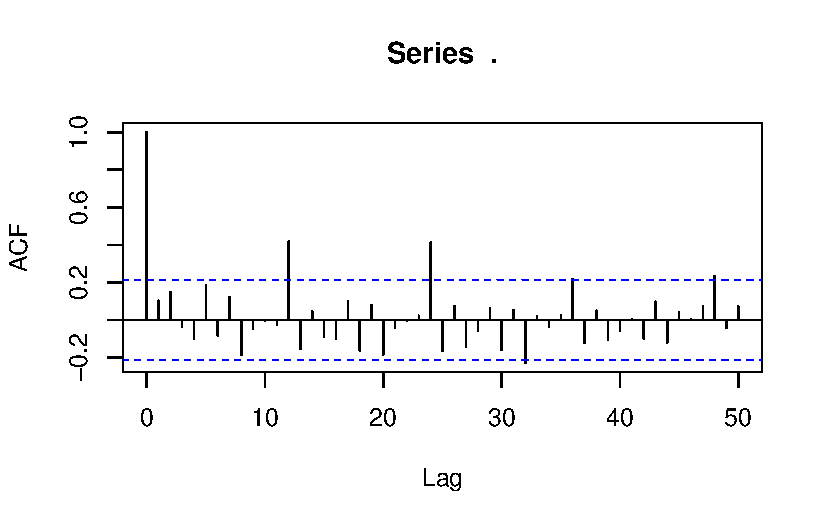
\includegraphics[keepaspectratio]{pre-covid-model_files/figure-pdf/unnamed-chunk-3-1.pdf}}

Initial visualizations show some signs of a seasonality with a regular
high around te winter periods. It does show a sligth quadratic trend but
is not very pronounced from this visualization, it shows high levels of
variability therefore we will consider the log of the series.

\begin{Shaded}
\begin{Highlighting}[]
\CommentTok{\# Create time series for each serires}

\NormalTok{df }\OtherTok{\textless{}{-}}\NormalTok{ df }\SpecialCharTok{\%\textgreater{}\%} 
    \FunctionTok{mutate}\NormalTok{(}
        \AttributeTok{data.ts =} \FunctionTok{map}\NormalTok{(}
            \AttributeTok{.x =}\NormalTok{ data,}
            \AttributeTok{.f =}\NormalTok{ tk\_ts,}
            \AttributeTok{select   =} \FunctionTok{c}\NormalTok{(}\SpecialCharTok{{-}}\NormalTok{data, }\SpecialCharTok{{-}}\NormalTok{year, }\SpecialCharTok{{-}}\NormalTok{urgencias\_geral),}
            \AttributeTok{start =} \DecValTok{2013}\NormalTok{,}
            \AttributeTok{freq =} \DecValTok{12}
\NormalTok{        )}
\NormalTok{    )}
\end{Highlighting}
\end{Shaded}

\begin{verbatim}
Warning: There were 2 warnings in `mutate()`.
The first warning was:
i In argument: `data.ts = map(...)`.
i In group 1: `unidade_saude = "Barcelos"`.
Caused by warning:
! Non-numeric columns being dropped: instituicao
i Run `dplyr::last_dplyr_warnings()` to see the 1 remaining warning.
\end{verbatim}

\begin{Shaded}
\begin{Highlighting}[]
\NormalTok{df}
\end{Highlighting}
\end{Shaded}

\begin{verbatim}
# A tibble: 2 x 3
# Groups:   unidade_saude [2]
  unidade_saude data              data.ts      
  <chr>         <list>            <list>       
1 Barcelos      <tibble [84 x 5]> <ts [84 x 1]>
2 Vila do Conde <tibble [84 x 5]> <ts [84 x 1]>
\end{verbatim}

\begin{Shaded}
\begin{Highlighting}[]
\NormalTok{df }\SpecialCharTok{\%\textgreater{}\%} 
    \FunctionTok{filter}\NormalTok{(unidade\_saude }\SpecialCharTok{==} \StringTok{"Vila do Conde"}\NormalTok{) }\SpecialCharTok{\%\textgreater{}\%}
    \FunctionTok{pull}\NormalTok{(data.ts) }\SpecialCharTok{\%\textgreater{}\%} 
\NormalTok{    .[[}\DecValTok{1}\NormalTok{]] }\SpecialCharTok{\%\textgreater{}\%} 
    \FunctionTok{decompose}\NormalTok{(}\AttributeTok{type =} \StringTok{"additive"}\NormalTok{) }\SpecialCharTok{\%\textgreater{}\%} 
    \FunctionTok{autoplot}\NormalTok{() }\SpecialCharTok{+}
    \FunctionTok{ggtitle}\NormalTok{(}\StringTok{"Vila do Conde"}\NormalTok{)}
\end{Highlighting}
\end{Shaded}

\pandocbounded{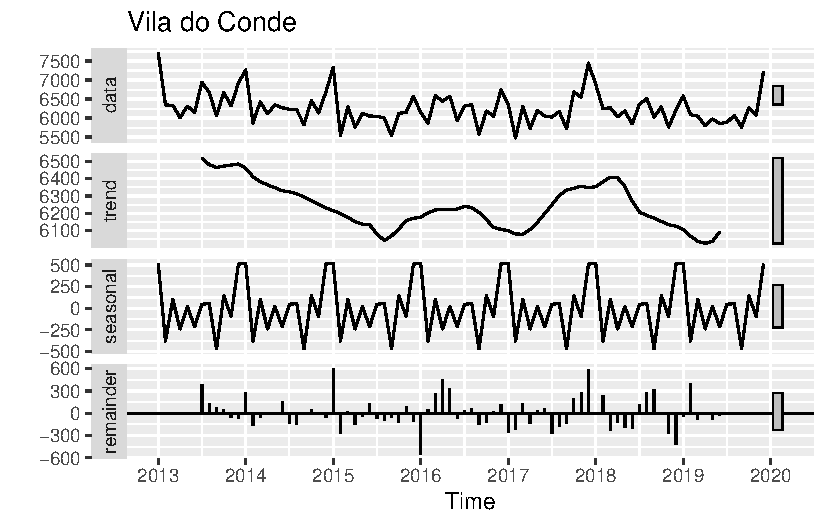
\includegraphics[keepaspectratio]{pre-covid-model_files/figure-pdf/unnamed-chunk-5-1.pdf}}

\begin{Shaded}
\begin{Highlighting}[]
\NormalTok{df }\SpecialCharTok{\%\textgreater{}\%} 
    \FunctionTok{filter}\NormalTok{(unidade\_saude }\SpecialCharTok{==} \StringTok{"Barcelos"}\NormalTok{) }\SpecialCharTok{\%\textgreater{}\%}
    \FunctionTok{pull}\NormalTok{(data.ts) }\SpecialCharTok{\%\textgreater{}\%} 
\NormalTok{    .[[}\DecValTok{1}\NormalTok{]] }\SpecialCharTok{\%\textgreater{}\%} 
    \FunctionTok{decompose}\NormalTok{(}\AttributeTok{type =} \StringTok{"additive"}\NormalTok{) }\SpecialCharTok{\%\textgreater{}\%} 
    \FunctionTok{autoplot}\NormalTok{() }\SpecialCharTok{+}
    \FunctionTok{ggtitle}\NormalTok{(}\StringTok{"Vila do Conde"}\NormalTok{)}
\end{Highlighting}
\end{Shaded}

\pandocbounded{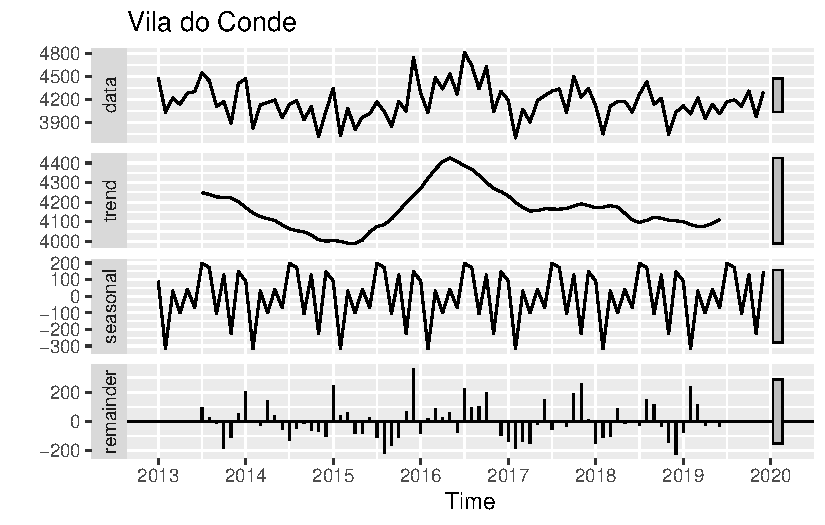
\includegraphics[keepaspectratio]{pre-covid-model_files/figure-pdf/unnamed-chunk-6-1.pdf}}

\subsection{Reducing variability}\label{reducing-variability}

\begin{Shaded}
\begin{Highlighting}[]
\NormalTok{df\_transform }\OtherTok{\textless{}{-}}\NormalTok{ df }\SpecialCharTok{\%\textgreater{}\%} 
    \FunctionTok{mutate}\NormalTok{(}
        \AttributeTok{boxcox.lambda =} \FunctionTok{map}\NormalTok{(data.ts, BoxCox.lambda),}
        \AttributeTok{data.ts.box =} \FunctionTok{map2}\NormalTok{(}
            \AttributeTok{.x =}\NormalTok{ data.ts,}
            \AttributeTok{.y =}\NormalTok{ boxcox.lambda,}
            \AttributeTok{.f =} \SpecialCharTok{\textasciitilde{}}\FunctionTok{BoxCox}\NormalTok{(.x, .y))}
\NormalTok{        )}
\end{Highlighting}
\end{Shaded}

\begin{Shaded}
\begin{Highlighting}[]
\NormalTok{df\_transform  }\SpecialCharTok{\%\textgreater{}\%} 
    \FunctionTok{filter}\NormalTok{(unidade\_saude }\SpecialCharTok{==} \StringTok{"Barcelos"}\NormalTok{) }\SpecialCharTok{\%\textgreater{}\%}
    \FunctionTok{pull}\NormalTok{(data.ts.box) }\SpecialCharTok{\%\textgreater{}\%} 
\NormalTok{    .[[}\DecValTok{1}\NormalTok{]] }\SpecialCharTok{\%\textgreater{}\%} 
    \FunctionTok{autoplot}\NormalTok{()}
\end{Highlighting}
\end{Shaded}

\pandocbounded{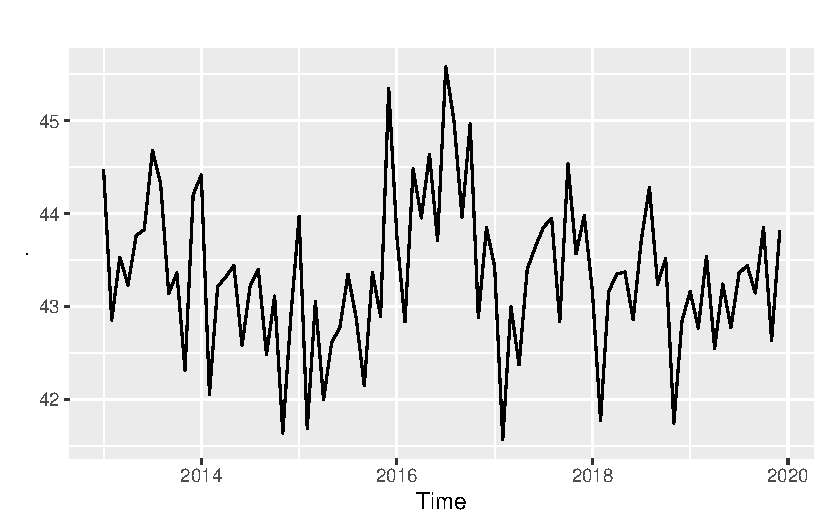
\includegraphics[keepaspectratio]{pre-covid-model_files/figure-pdf/unnamed-chunk-8-1.pdf}}

\begin{Shaded}
\begin{Highlighting}[]
\NormalTok{df\_transform }\OtherTok{\textless{}{-}}\NormalTok{ df\_transform }\SpecialCharTok{\%\textgreater{}\%} 
    \FunctionTok{mutate}\NormalTok{(}
        \AttributeTok{stat.diffseason =} \FunctionTok{map}\NormalTok{(}\AttributeTok{.x =}\NormalTok{ data.ts.box, nsdiffs),}
        \AttributeTok{stat.diff6 =} \FunctionTok{map}\NormalTok{(}\AttributeTok{.x =}\NormalTok{ data.ts.box,}\AttributeTok{.f =} \SpecialCharTok{\textasciitilde{}}\FunctionTok{ndiffs}\NormalTok{(}\FunctionTok{diff}\NormalTok{(.x, }\DecValTok{6}\NormalTok{))),}
        \AttributeTok{stat.diff12 =} \FunctionTok{map}\NormalTok{(}\AttributeTok{.x =}\NormalTok{ data.ts.box,}\AttributeTok{.f =} \SpecialCharTok{\textasciitilde{}}\FunctionTok{ndiffs}\NormalTok{(}\FunctionTok{diff}\NormalTok{(.x, }\DecValTok{12}\NormalTok{))),}
        \AttributeTok{diff1 =} \FunctionTok{map}\NormalTok{(}\AttributeTok{.x =}\NormalTok{ data.ts.box, }\AttributeTok{.f =} \SpecialCharTok{\textasciitilde{}}\FunctionTok{diff}\NormalTok{(.x, }\DecValTok{1}\NormalTok{)),}
        \AttributeTok{diff6 =} \FunctionTok{map}\NormalTok{(}\AttributeTok{.x =}\NormalTok{ data.ts.box, }\AttributeTok{.f =} \SpecialCharTok{\textasciitilde{}}\FunctionTok{diff}\NormalTok{(.x, }\DecValTok{6}\NormalTok{)),}
        \AttributeTok{diff12 =} \FunctionTok{map}\NormalTok{(}\AttributeTok{.x =}\NormalTok{ data.ts.box, }\AttributeTok{.f =} \SpecialCharTok{\textasciitilde{}}\FunctionTok{diff}\NormalTok{(.x, }\DecValTok{12}\NormalTok{)),}
        \AttributeTok{diff6.1 =} \FunctionTok{map}\NormalTok{(}\AttributeTok{.x =}\NormalTok{ data.ts.box, }\AttributeTok{.f =} \SpecialCharTok{\textasciitilde{}}\FunctionTok{diff}\NormalTok{(}\FunctionTok{diff}\NormalTok{(.x, }\DecValTok{6}\NormalTok{),}\DecValTok{1}\NormalTok{)),}
        \AttributeTok{diff12.1 =} \FunctionTok{map}\NormalTok{(}\AttributeTok{.x =}\NormalTok{ data.ts.box, }\AttributeTok{.f =} \SpecialCharTok{\textasciitilde{}}\FunctionTok{diff}\NormalTok{(}\FunctionTok{diff}\NormalTok{(.x, }\DecValTok{12}\NormalTok{),}\DecValTok{1}\NormalTok{))}
\NormalTok{    )}
\end{Highlighting}
\end{Shaded}

\begin{Shaded}
\begin{Highlighting}[]
\NormalTok{pl1 }\OtherTok{\textless{}{-}}\NormalTok{ df\_transform  }\SpecialCharTok{\%\textgreater{}\%} 
    \FunctionTok{filter}\NormalTok{(unidade\_saude }\SpecialCharTok{==} \StringTok{"Vila do Conde"}\NormalTok{) }\SpecialCharTok{\%\textgreater{}\%}
    \FunctionTok{pull}\NormalTok{(data.ts.box) }\SpecialCharTok{\%\textgreater{}\%} 
\NormalTok{    .[[}\DecValTok{1}\NormalTok{]] }\SpecialCharTok{\%\textgreater{}\%} 
    \FunctionTok{autoplot}\NormalTok{() }\SpecialCharTok{+} 
    \FunctionTok{ggtitle}\NormalTok{(}\StringTok{"Vila do conde"}\NormalTok{)}


\NormalTok{pl2 }\OtherTok{\textless{}{-}}\NormalTok{ df\_transform  }\SpecialCharTok{\%\textgreater{}\%} 
    \FunctionTok{filter}\NormalTok{(unidade\_saude }\SpecialCharTok{==} \StringTok{"Vila do Conde"}\NormalTok{) }\SpecialCharTok{\%\textgreater{}\%}
    \FunctionTok{pull}\NormalTok{(diff1) }\SpecialCharTok{\%\textgreater{}\%} 
\NormalTok{    .[[}\DecValTok{1}\NormalTok{]] }\SpecialCharTok{\%\textgreater{}\%} 
    \FunctionTok{autoplot}\NormalTok{() }\SpecialCharTok{+} 
    \FunctionTok{ggtitle}\NormalTok{(}\StringTok{"Vila do conde diff1"}\NormalTok{)}

\NormalTok{pl3 }\OtherTok{\textless{}{-}}\NormalTok{ df\_transform  }\SpecialCharTok{\%\textgreater{}\%} 
    \FunctionTok{filter}\NormalTok{(unidade\_saude }\SpecialCharTok{==} \StringTok{"Vila do Conde"}\NormalTok{) }\SpecialCharTok{\%\textgreater{}\%}
    \FunctionTok{pull}\NormalTok{(diff6) }\SpecialCharTok{\%\textgreater{}\%} 
\NormalTok{    .[[}\DecValTok{1}\NormalTok{]] }\SpecialCharTok{\%\textgreater{}\%} 
    \FunctionTok{autoplot}\NormalTok{() }\SpecialCharTok{+} 
    \FunctionTok{ggtitle}\NormalTok{(}\StringTok{"Vila do conde diff6"}\NormalTok{)}

\NormalTok{pl4 }\OtherTok{\textless{}{-}}\NormalTok{ df\_transform  }\SpecialCharTok{\%\textgreater{}\%} 
    \FunctionTok{filter}\NormalTok{(unidade\_saude }\SpecialCharTok{==} \StringTok{"Vila do Conde"}\NormalTok{) }\SpecialCharTok{\%\textgreater{}\%}
    \FunctionTok{pull}\NormalTok{(diff12) }\SpecialCharTok{\%\textgreater{}\%} 
\NormalTok{    .[[}\DecValTok{1}\NormalTok{]] }\SpecialCharTok{\%\textgreater{}\%} 
    \FunctionTok{autoplot}\NormalTok{() }\SpecialCharTok{+} 
    \FunctionTok{ggtitle}\NormalTok{(}\StringTok{"Vila do conde diff12"}\NormalTok{)}

\NormalTok{pl5 }\OtherTok{\textless{}{-}}\NormalTok{ df\_transform  }\SpecialCharTok{\%\textgreater{}\%} 
    \FunctionTok{filter}\NormalTok{(unidade\_saude }\SpecialCharTok{==} \StringTok{"Vila do Conde"}\NormalTok{) }\SpecialCharTok{\%\textgreater{}\%}
    \FunctionTok{pull}\NormalTok{(diff6}\FloatTok{.1}\NormalTok{) }\SpecialCharTok{\%\textgreater{}\%} 
\NormalTok{    .[[}\DecValTok{1}\NormalTok{]] }\SpecialCharTok{\%\textgreater{}\%} 
    \FunctionTok{autoplot}\NormalTok{() }\SpecialCharTok{+} 
    \FunctionTok{ggtitle}\NormalTok{(}\StringTok{"Vila do conde diff6.1"}\NormalTok{)}

\NormalTok{pl6 }\OtherTok{\textless{}{-}}\NormalTok{ df\_transform  }\SpecialCharTok{\%\textgreater{}\%} 
    \FunctionTok{filter}\NormalTok{(unidade\_saude }\SpecialCharTok{==} \StringTok{"Vila do Conde"}\NormalTok{) }\SpecialCharTok{\%\textgreater{}\%}
    \FunctionTok{pull}\NormalTok{(diff12}\FloatTok{.1}\NormalTok{) }\SpecialCharTok{\%\textgreater{}\%} 
\NormalTok{    .[[}\DecValTok{1}\NormalTok{]] }\SpecialCharTok{\%\textgreater{}\%} 
    \FunctionTok{autoplot}\NormalTok{() }\SpecialCharTok{+} 
    \FunctionTok{ggtitle}\NormalTok{(}\StringTok{"Vila do conde diff12.1"}\NormalTok{)}

\FunctionTok{grid.arrange}\NormalTok{(pl1,pl2,pl3,pl4,pl5,pl6, }\AttributeTok{ncol =} \DecValTok{2}\NormalTok{)}
\end{Highlighting}
\end{Shaded}

\pandocbounded{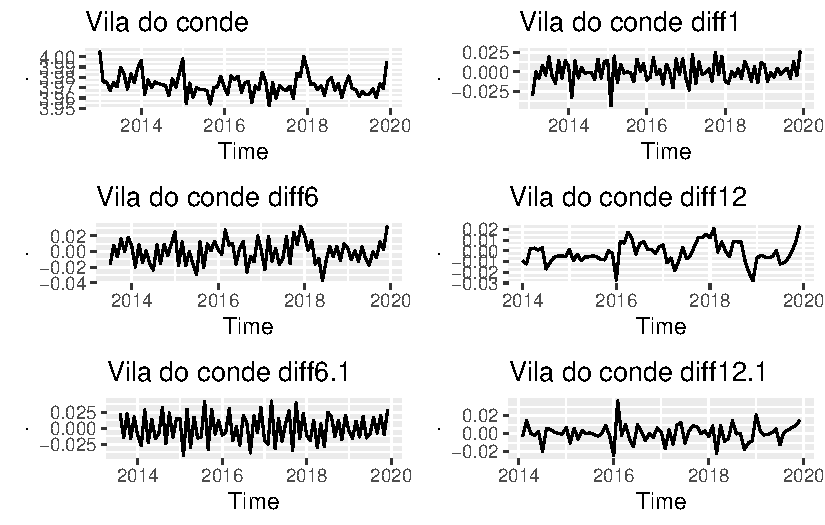
\includegraphics[keepaspectratio]{pre-covid-model_files/figure-pdf/unnamed-chunk-10-1.pdf}}

\begin{Shaded}
\begin{Highlighting}[]
\NormalTok{acf1 }\OtherTok{\textless{}{-}}\NormalTok{ df\_transform  }\SpecialCharTok{\%\textgreater{}\%} 
    \FunctionTok{filter}\NormalTok{(unidade\_saude }\SpecialCharTok{==} \StringTok{"Vila do Conde"}\NormalTok{) }\SpecialCharTok{\%\textgreater{}\%}
    \FunctionTok{pull}\NormalTok{(data.ts.box) }\SpecialCharTok{\%\textgreater{}\%} 
\NormalTok{    .[[}\DecValTok{1}\NormalTok{]] }\SpecialCharTok{\%\textgreater{}\%} 
    \FunctionTok{ggtsdisplay}\NormalTok{(}\AttributeTok{main =} \StringTok{"Vila do Conde"}\NormalTok{)}
\end{Highlighting}
\end{Shaded}

\pandocbounded{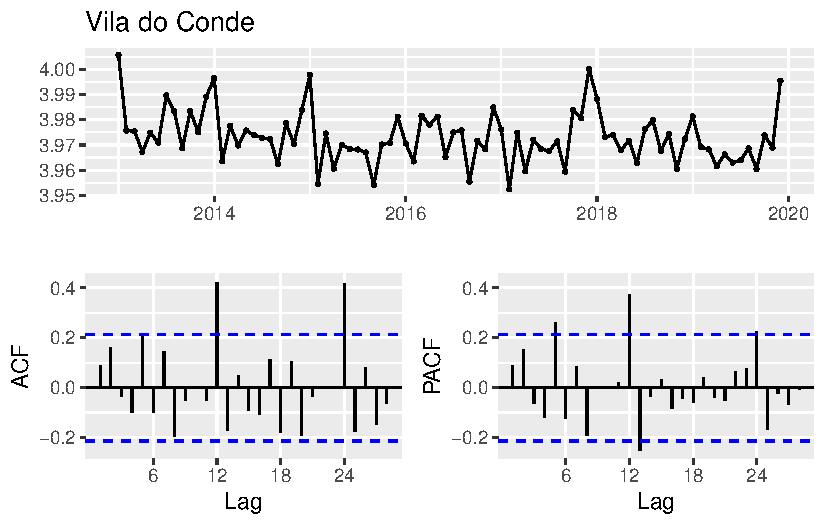
\includegraphics[keepaspectratio]{pre-covid-model_files/figure-pdf/unnamed-chunk-11-1.pdf}}

\begin{Shaded}
\begin{Highlighting}[]
\NormalTok{acf2 }\OtherTok{\textless{}{-}}\NormalTok{ df\_transform  }\SpecialCharTok{\%\textgreater{}\%} 
    \FunctionTok{filter}\NormalTok{(unidade\_saude }\SpecialCharTok{==} \StringTok{"Vila do Conde"}\NormalTok{) }\SpecialCharTok{\%\textgreater{}\%}
    \FunctionTok{pull}\NormalTok{(diff1) }\SpecialCharTok{\%\textgreater{}\%} 
\NormalTok{    .[[}\DecValTok{1}\NormalTok{]] }\SpecialCharTok{\%\textgreater{}\%}
    \FunctionTok{ggtsdisplay}\NormalTok{(}\AttributeTok{main =} \StringTok{"Vila do Conde diff1"}\NormalTok{)}
\end{Highlighting}
\end{Shaded}

\pandocbounded{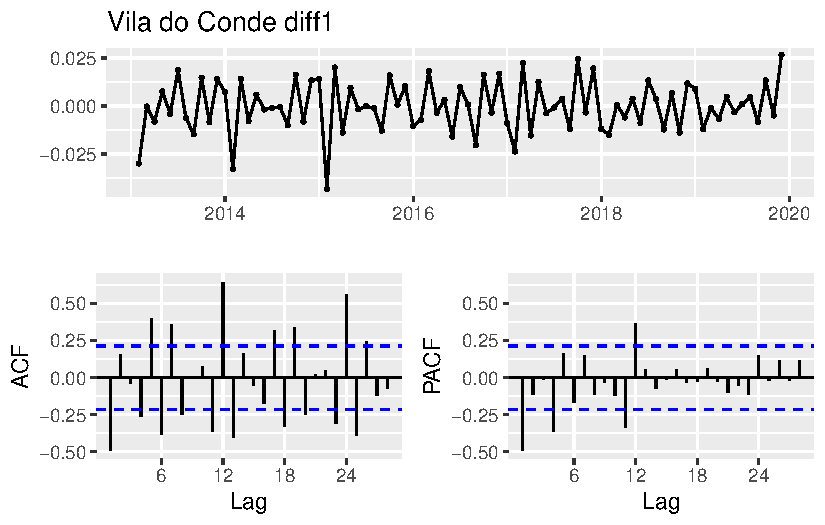
\includegraphics[keepaspectratio]{pre-covid-model_files/figure-pdf/unnamed-chunk-11-2.pdf}}

\begin{Shaded}
\begin{Highlighting}[]
\NormalTok{acf3 }\OtherTok{\textless{}{-}}\NormalTok{ df\_transform  }\SpecialCharTok{\%\textgreater{}\%} 
    \FunctionTok{filter}\NormalTok{(unidade\_saude }\SpecialCharTok{==} \StringTok{"Vila do Conde"}\NormalTok{) }\SpecialCharTok{\%\textgreater{}\%}
    \FunctionTok{pull}\NormalTok{(diff6) }\SpecialCharTok{\%\textgreater{}\%} 
\NormalTok{    .[[}\DecValTok{1}\NormalTok{]] }\SpecialCharTok{\%\textgreater{}\%} 
    \FunctionTok{ggtsdisplay}\NormalTok{(}\AttributeTok{main =} \StringTok{"Vila do Conde diff6"}\NormalTok{)}
\end{Highlighting}
\end{Shaded}

\pandocbounded{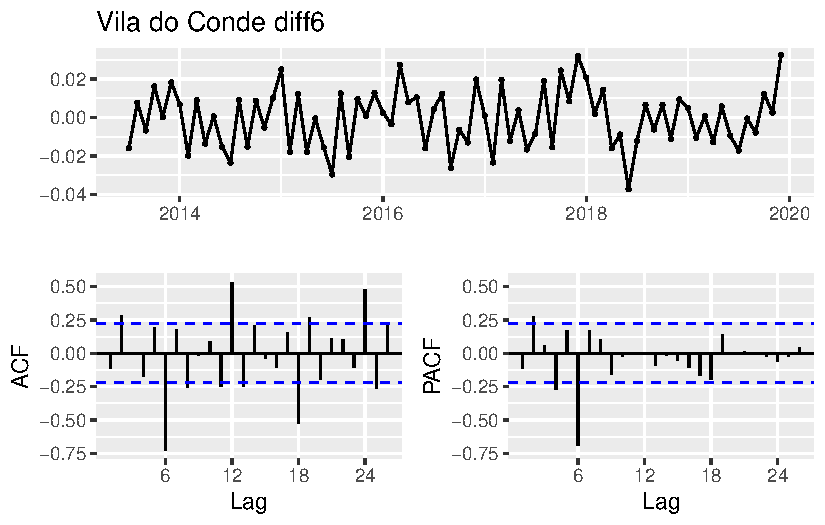
\includegraphics[keepaspectratio]{pre-covid-model_files/figure-pdf/unnamed-chunk-11-3.pdf}}

\begin{Shaded}
\begin{Highlighting}[]
\NormalTok{acf4 }\OtherTok{\textless{}{-}}\NormalTok{ df\_transform  }\SpecialCharTok{\%\textgreater{}\%} 
    \FunctionTok{filter}\NormalTok{(unidade\_saude }\SpecialCharTok{==} \StringTok{"Vila do Conde"}\NormalTok{) }\SpecialCharTok{\%\textgreater{}\%}
    \FunctionTok{pull}\NormalTok{(diff12) }\SpecialCharTok{\%\textgreater{}\%} 
\NormalTok{    .[[}\DecValTok{1}\NormalTok{]] }\SpecialCharTok{\%\textgreater{}\%} 
    \FunctionTok{ggtsdisplay}\NormalTok{(}\AttributeTok{main =} \StringTok{"Vila do Conde diff12"}\NormalTok{)}
\end{Highlighting}
\end{Shaded}

\pandocbounded{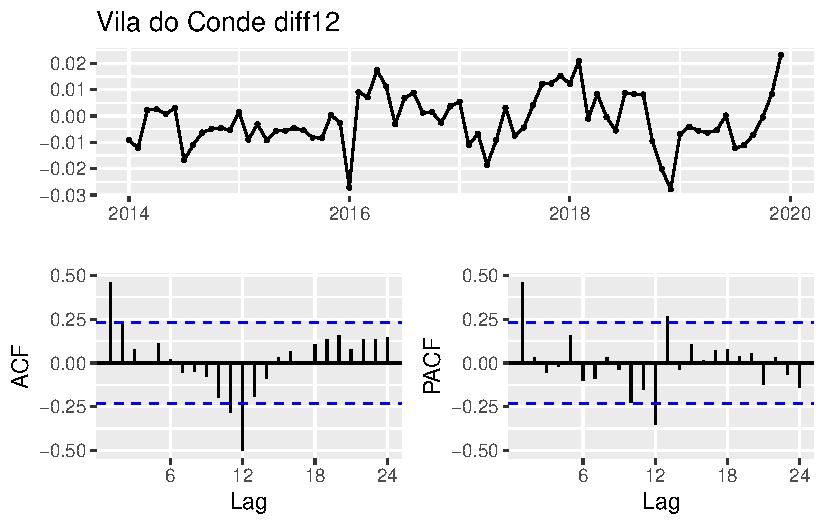
\includegraphics[keepaspectratio]{pre-covid-model_files/figure-pdf/unnamed-chunk-11-4.pdf}}

\begin{Shaded}
\begin{Highlighting}[]
\NormalTok{acf5 }\OtherTok{\textless{}{-}}\NormalTok{ df\_transform  }\SpecialCharTok{\%\textgreater{}\%} 
    \FunctionTok{filter}\NormalTok{(unidade\_saude }\SpecialCharTok{==} \StringTok{"Vila do Conde"}\NormalTok{) }\SpecialCharTok{\%\textgreater{}\%}
    \FunctionTok{pull}\NormalTok{(diff6}\FloatTok{.1}\NormalTok{) }\SpecialCharTok{\%\textgreater{}\%} 
\NormalTok{    .[[}\DecValTok{1}\NormalTok{]] }\SpecialCharTok{\%\textgreater{}\%} 
    \FunctionTok{ggtsdisplay}\NormalTok{(}\AttributeTok{main =} \StringTok{"Vila do Conde diff6.1"}\NormalTok{)}
\end{Highlighting}
\end{Shaded}

\pandocbounded{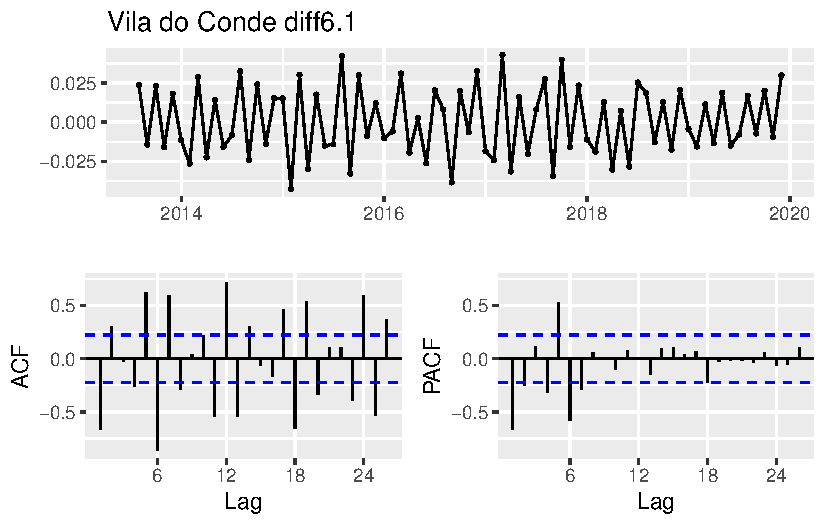
\includegraphics[keepaspectratio]{pre-covid-model_files/figure-pdf/unnamed-chunk-11-5.pdf}}

\begin{Shaded}
\begin{Highlighting}[]
\NormalTok{acf6 }\OtherTok{\textless{}{-}}\NormalTok{ df\_transform  }\SpecialCharTok{\%\textgreater{}\%} 
    \FunctionTok{filter}\NormalTok{(unidade\_saude }\SpecialCharTok{==} \StringTok{"Vila do Conde"}\NormalTok{) }\SpecialCharTok{\%\textgreater{}\%}
    \FunctionTok{pull}\NormalTok{(diff12}\FloatTok{.1}\NormalTok{) }\SpecialCharTok{\%\textgreater{}\%} 
\NormalTok{    .[[}\DecValTok{1}\NormalTok{]] }\SpecialCharTok{\%\textgreater{}\%} 
    \FunctionTok{ggtsdisplay}\NormalTok{(}\AttributeTok{main =} \StringTok{"Vila do Conde diff12.1"}\NormalTok{)}
\end{Highlighting}
\end{Shaded}

\pandocbounded{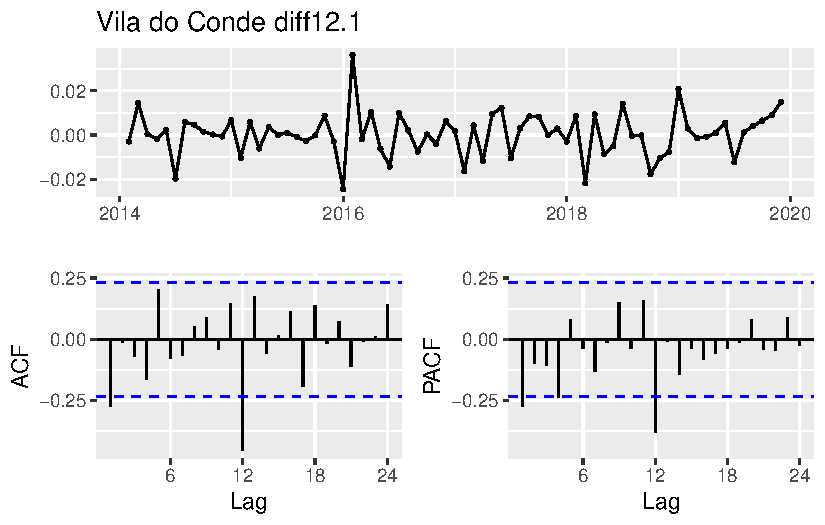
\includegraphics[keepaspectratio]{pre-covid-model_files/figure-pdf/unnamed-chunk-11-6.pdf}}

\subsection{Split data}\label{split-data}

\begin{Shaded}
\begin{Highlighting}[]
\NormalTok{df\_train\_test }\OtherTok{\textless{}{-}}\NormalTok{ df\_transform }\SpecialCharTok{\%\textgreater{}\%} 
    \FunctionTok{mutate}\NormalTok{(}
        \AttributeTok{train =} \FunctionTok{map}\NormalTok{(}
            \AttributeTok{.x =}\NormalTok{ diff1,}
            \AttributeTok{.f =} \SpecialCharTok{\textasciitilde{}}\FunctionTok{window}\NormalTok{(.x, }\AttributeTok{end =} \FunctionTok{c}\NormalTok{(}\DecValTok{2019}\NormalTok{, }\DecValTok{10}\NormalTok{))}
\NormalTok{        ),}
        \AttributeTok{test =} \FunctionTok{map}\NormalTok{(}
            \AttributeTok{.x =}\NormalTok{ diff1,}
            \AttributeTok{.f =} \SpecialCharTok{\textasciitilde{}}\FunctionTok{window}\NormalTok{(.x, }\AttributeTok{start =} \FunctionTok{c}\NormalTok{(}\DecValTok{2019}\NormalTok{, }\DecValTok{11}\NormalTok{)) }
\NormalTok{        )}
\NormalTok{    )}

\NormalTok{df\_train\_test}
\end{Highlighting}
\end{Shaded}

\begin{verbatim}
# A tibble: 2 x 15
# Groups:   unidade_saude [2]
  unidade_saude data     data.ts       boxcox.lambda data.ts.box stat.diffseason
  <chr>         <list>   <list>        <list>        <list>      <list>         
1 Barcelos      <tibble> <ts [84 x 1]> <dbl [1]>     <ts[...]>   <dbl [1]>      
2 Vila do Conde <tibble> <ts [84 x 1]> <dbl [1]>     <ts[...]>   <dbl [1]>      
# i 9 more variables: stat.diff6 <list>, stat.diff12 <list>, diff1 <list>,
#   diff6 <list>, diff12 <list>, diff6.1 <list>, diff12.1 <list>, train <list>,
#   test <list>
\end{verbatim}

\begin{Shaded}
\begin{Highlighting}[]
\NormalTok{tr\_pl }\OtherTok{\textless{}{-}}\NormalTok{ df\_train\_test }\SpecialCharTok{\%\textgreater{}\%} 
    \FunctionTok{filter}\NormalTok{(unidade\_saude }\SpecialCharTok{==} \StringTok{"Vila do Conde"}\NormalTok{) }\SpecialCharTok{\%\textgreater{}\%}
    \FunctionTok{pull}\NormalTok{(train) }\SpecialCharTok{\%\textgreater{}\%} 
\NormalTok{    .[[}\DecValTok{1}\NormalTok{]] }\SpecialCharTok{\%\textgreater{}\%} 
    \FunctionTok{autoplot}\NormalTok{()}

\NormalTok{layer }\OtherTok{\textless{}{-}}\NormalTok{ df\_train\_test }\SpecialCharTok{\%\textgreater{}\%} 
    \FunctionTok{filter}\NormalTok{(unidade\_saude }\SpecialCharTok{==} \StringTok{"Vila do Conde"}\NormalTok{) }\SpecialCharTok{\%\textgreater{}\%}
    \FunctionTok{pull}\NormalTok{(test) }\SpecialCharTok{\%\textgreater{}\%} 
\NormalTok{    .[[}\DecValTok{1}\NormalTok{]] }\SpecialCharTok{\%\textgreater{}\%} 
    \FunctionTok{autolayer}\NormalTok{()}

\NormalTok{tr\_pl }\SpecialCharTok{+}\NormalTok{ layer}
\end{Highlighting}
\end{Shaded}

\pandocbounded{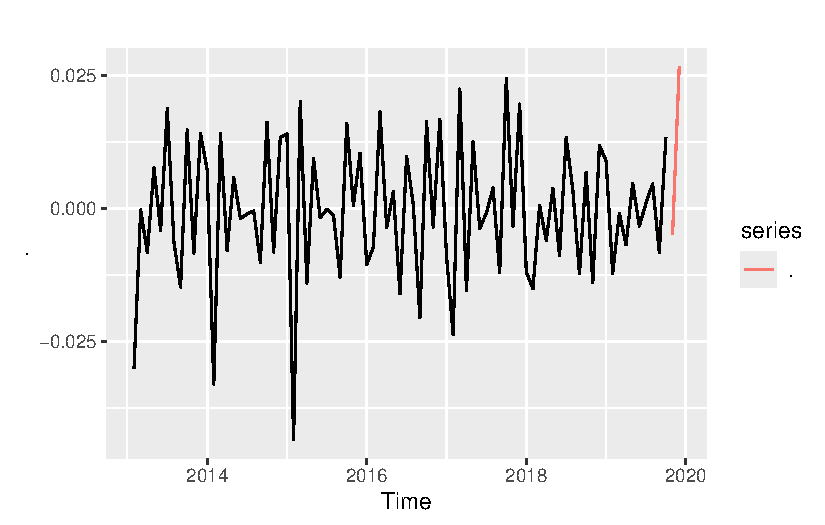
\includegraphics[keepaspectratio]{pre-covid-model_files/figure-pdf/unnamed-chunk-13-1.pdf}}

\begin{Shaded}
\begin{Highlighting}[]
\FunctionTok{kpss.test}\NormalTok{(df\_transform}\SpecialCharTok{$}\NormalTok{diff1[[}\DecValTok{1}\NormalTok{]])}
\end{Highlighting}
\end{Shaded}

\begin{verbatim}
Warning in kpss.test(df_transform$diff1[[1]]): p-value greater than printed
p-value
\end{verbatim}

\begin{verbatim}

    KPSS Test for Level Stationarity

data:  df_transform$diff1[[1]]
KPSS Level = 0.048206, Truncation lag parameter = 3, p-value = 0.1
\end{verbatim}

\begin{Shaded}
\begin{Highlighting}[]
\FunctionTok{adf.test}\NormalTok{(df\_transform}\SpecialCharTok{$}\NormalTok{diff1[[}\DecValTok{1}\NormalTok{]])}
\end{Highlighting}
\end{Shaded}

\begin{verbatim}
Warning in adf.test(df_transform$diff1[[1]]): p-value smaller than printed
p-value
\end{verbatim}

\begin{verbatim}

    Augmented Dickey-Fuller Test

data:  df_transform$diff1[[1]]
Dickey-Fuller = -4.7912, Lag order = 4, p-value = 0.01
alternative hypothesis: stationary
\end{verbatim}

\begin{Shaded}
\begin{Highlighting}[]
\NormalTok{df\_train\_test }\OtherTok{\textless{}{-}}\NormalTok{ df\_train\_test }\SpecialCharTok{\%\textgreater{}\%} 
    \FunctionTok{mutate}\NormalTok{(}
        \AttributeTok{model.fit =} \FunctionTok{map}\NormalTok{(}\AttributeTok{.x =}\NormalTok{ train, }\SpecialCharTok{\textasciitilde{}}\FunctionTok{auto.arima}\NormalTok{(.x)),}
        \AttributeTok{test.forecast =} \FunctionTok{map2}\NormalTok{(}\AttributeTok{.x =}\NormalTok{ model.fit ,}\AttributeTok{.y =}\NormalTok{ test , }\AttributeTok{.f =} \SpecialCharTok{\textasciitilde{}}\FunctionTok{forecast}\NormalTok{(.x, }\AttributeTok{h =} \FunctionTok{length}\NormalTok{(.y))),}
        \AttributeTok{test.mse =} \FunctionTok{map2}\NormalTok{(}\AttributeTok{.x =}\NormalTok{ test.forecast , }\AttributeTok{.y =}\NormalTok{ test, }\AttributeTok{.f =} \SpecialCharTok{\textasciitilde{}}\FunctionTok{mean}\NormalTok{((.x}\SpecialCharTok{$}\NormalTok{mean }\SpecialCharTok{{-}}\NormalTok{ .y)}\SpecialCharTok{\^{}}\DecValTok{2}\NormalTok{)) }
\NormalTok{    )}
\end{Highlighting}
\end{Shaded}

\begin{Shaded}
\begin{Highlighting}[]
\NormalTok{t }\OtherTok{\textless{}{-}}\NormalTok{ df\_train\_test }\SpecialCharTok{\%\textgreater{}\%} 
    \FunctionTok{mutate}\NormalTok{(}
        \AttributeTok{forecast.covid =}  \FunctionTok{map}\NormalTok{(}\AttributeTok{.x =}\NormalTok{ model.fit, }\AttributeTok{.f =} \SpecialCharTok{\textasciitilde{}}\FunctionTok{forecast}\NormalTok{(.x, }\AttributeTok{h =} \DecValTok{22}\NormalTok{))}
\NormalTok{    )}

\NormalTok{t}\SpecialCharTok{$}\NormalTok{forecast.covid}
\end{Highlighting}
\end{Shaded}

\begin{verbatim}
[[1]]
         Point Forecast        Lo 80      Hi 80       Lo 95      Hi 95
Nov 2019   -1.324106638 -2.058526250 -0.5896870 -2.44730451 -0.2009088
Dec 2019    1.247806518  0.482168639  2.0134444  0.07686443  2.4187486
Jan 2020   -0.342447748 -1.117200488  0.4323050 -1.52732981  0.8424343
Feb 2020   -1.603740541 -2.377824681 -0.8296564 -2.78760007 -0.4198810
Mar 2020    1.282409259  0.507448847  2.0573697  0.09720959  2.4676089
Apr 2020   -0.391330883 -1.166561802  0.3839000 -1.57694426  0.7942825
May 2020    0.503631399 -0.271683056  1.2789459 -0.68210974  1.6893725
Jun 2020   -0.329212447 -1.104552664  0.4461278 -1.51499298  0.8565681
Jul 2020    0.808822616  0.033474581  1.5841707 -0.37696988  1.9946151
Aug 2020   -0.012292850 -0.787642846  0.7630571 -1.19808834  1.1735026
Sep 2020   -0.956298128 -1.731647261 -0.1809490 -2.14209230  0.2294960
Oct 2020    0.852463180  0.077119072  1.6278073 -0.33332331  2.0382497
Nov 2020   -1.348361464 -2.125542811 -0.5711801 -2.53695776 -0.1597652
Dec 2020    1.250530885  0.473248494  2.0278133  0.06178005  2.4392817
Jan 2021   -0.222354473 -0.999474718  0.5547658 -1.41085733  0.9661484
Feb 2021   -1.400788966 -2.175467319 -0.6261106 -2.58555727 -0.2160207
Mar 2021    1.205071633  0.430389396  1.9797539  0.02029739  2.3898459
Apr 2021   -0.485084150 -1.259767585  0.2895993 -1.66986022  0.6996919
May 2021    0.534890241 -0.239793555  1.3095740 -0.64988638  1.7196669
Jun 2021   -0.350805745 -1.125489621  0.4238781 -1.53558249  0.8339710
Jul 2021    0.773264686 -0.001419116  1.5479485 -0.41151195  1.9580413
Aug 2021    0.003320155 -0.771363304  0.7780036 -1.18145596  1.1880963

[[2]]
         Point Forecast        Lo 80        Hi 80        Lo 95        Hi 95
Nov 2019  -0.0072963594 -0.016366429  0.001773710 -0.021167834  0.006575115
Dec 2019   0.0144575476  0.004239139  0.024675956 -0.001170159  0.030085255
Jan 2020  -0.0000291316 -0.010396775  0.010338512 -0.015885074  0.015826811
Feb 2020  -0.0205561770 -0.030917319 -0.010195035 -0.036402176 -0.004710178
Mar 2020   0.0089258534 -0.001438550  0.019290257 -0.006925134  0.024776841
Apr 2020  -0.0085128345 -0.018877713  0.001852044 -0.024364549  0.007338880
May 2020   0.0064199755 -0.003944973  0.016784924 -0.009431845  0.022271796
Jun 2020  -0.0057872029 -0.016152161  0.004577755 -0.021639039  0.010064633
Jul 2020   0.0054321340 -0.004932826  0.015797094 -0.010419704  0.021283972
Aug 2020   0.0018613013 -0.008503658  0.012226261 -0.013990536  0.017713139
Sep 2020  -0.0122889011 -0.022653859 -0.001923943 -0.028140736  0.003562934
Oct 2020   0.0148457396  0.004480795  0.025210684 -0.001006075  0.030697554
Nov 2020  -0.0067833226 -0.017392174  0.003825529 -0.023008161  0.009441516
Dec 2020   0.0146533753  0.003980810  0.025325941 -0.001668905  0.030975655
Jan 2021   0.0000456164 -0.010628943  0.010720176 -0.016279713  0.016370946
Feb 2021  -0.0205276455 -0.031175819 -0.009879472 -0.036812622 -0.004242669
Mar 2021   0.0089367440 -0.001711618  0.019585106 -0.007348521  0.025222009
Apr 2021  -0.0085086775 -0.019157068  0.002139712 -0.024793985  0.007776630
May 2021   0.0064215623 -0.004226832  0.017069956 -0.009863751  0.022706876
Jun 2021  -0.0057865972 -0.016434992  0.004861797 -0.022071911  0.010498717
Jul 2021   0.0054323651 -0.005216029  0.016080760 -0.010852949  0.021717679
Aug 2021   0.0018613896 -0.008787005  0.012509784 -0.014423924  0.018146703
\end{verbatim}




\end{document}
